\documentclass{standalone}
\begin{document}
\subsection{Aufgabe 10.2}
Zunächst muss eine Funktion zur Bestimmung der Kantenlänge des inneren Quadrats aufgestellt werden. Da die Fläche eines Quadrats sich einfach aus dem Quadrat seiner Kantenlänge ergibt, reicht zur Minimierung des Flächeninhalts die Minimierung seiner Kantenlänge aus.
Legt man den Koordinatenursprung in den Mittelpunkt des äußeren Quadrats wird deutlich, dass die Punkte das inneren Quadrats stets durch Rotationen um 90° um den Ursprung gebildet werden. Dazu liegen sie immer auf der Kante des äußeren Quadrats, sodass eine Koordinate stets $\pm \frac{L}{2}$ beträgt.
Somit haben wir nur eine freie Koordinate zur Verfügung, die das Quadrat vollständig definiert, in diesem Fall $x$ genannt.
$x$ beschreibt den horizontalen Abstand des oberen Punkts des inneren Quadrats vom Koordinatenursprung.

\begin{figure}[htbp]
    \centering
    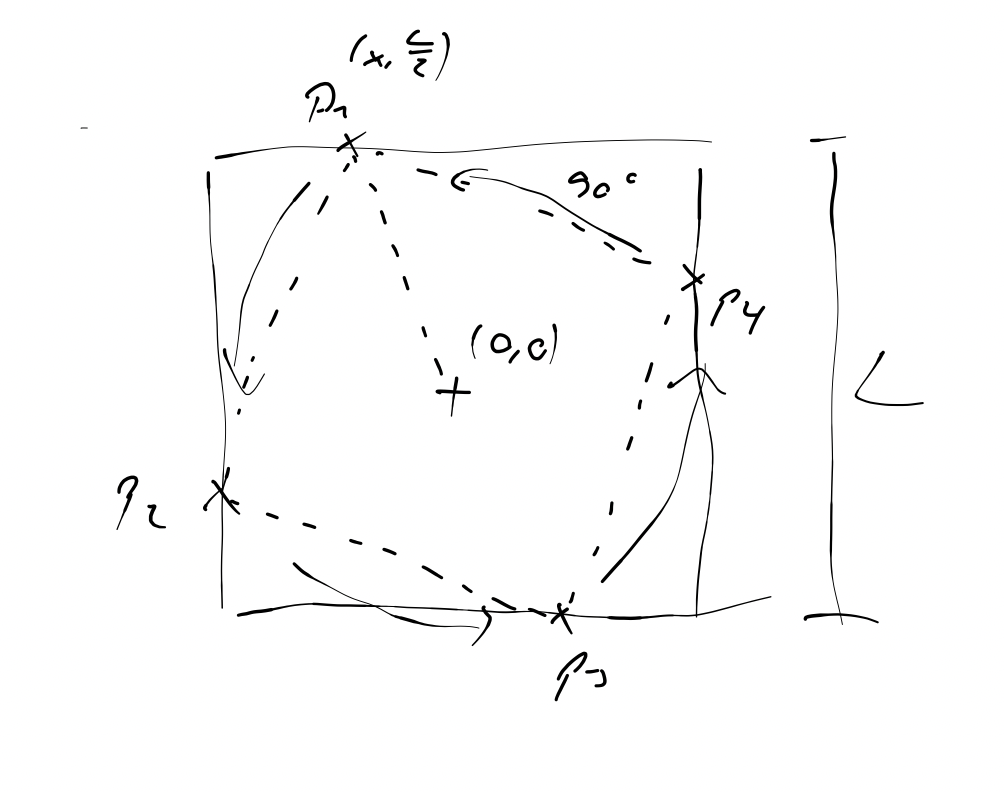
\includegraphics[width=10cm]{10_2.png}
\end{figure}

Für die Eckpunkte $p_i$ des inneren Quadrats ergibt sich damit:
\begin{align}
    p_1 &= (x, \frac{L}{2})^T \\
    p_2 &= (-\frac{L}{2}, x)^T \\
    p_3 &= (-x, -\frac{L}{2})^T \\
    p_4 &= (\frac{L}{2}, -x)^T
\end{align}
Zur Bestimmung der Kantenlänge des inneren Quadrats genügt die Berechnung des Abstands zweier nebeinanderliegender Punkte.
\begin{align}
    \abs{\overrightarrow{p_1 p_2}} &= \abs{(-x -\frac{L}{2}, -\frac{L}{2} + x)^T} \\
    &= \sqrt{(x+\frac{L}{2})^2 + (\frac{L}{2} - x)^2} \\
    &= \sqrt{f(x)}
\end{align}

Zur Minimierung der Kantenlänge reicht die Minimierung der Funktion $f(x)$ unter der Wurzel aus.

\begin{align}
    f(x) &= x^2 + \frac{L^2}{4} + x^2 + \frac{L^2}{4} \\
    &= 2x^2 + \frac{L^2}{2} \\
    \\
    f'(x) = 4x &= 0 \\
    x &= 0\\
    f''(x=0) &= 4 \geq 0 \text{, also Minimum} \\
    \\
    f(0) &= \frac{L^2}{2} \\
    f(\frac{L}{2}) &= L^2 \text{, Test der Bereichsgrenzen für } x
\end{align}

Zur Berechnung der Kantenlänge wird noch die Wurzel aus $f(0)$ gezogen, also

$$l_min = \sqrt{f(0)} = \frac{\sqrt{2}}{2} L$$



\end{document}